\chapter{Fuzzy Ontology Based Model evaluation and benchmarks} 

\section{Introduction}
		In order to illustrate the semantic enhancement of concept detection introduced 
		by our proposed ontology-based framework, we have conducted two preliminary experiments within two 
		multimedia evaluation campaigns. Hence, we first expose the experimental setup and the 
		obtained results of our framework within Trec Video Retrieval Evaluation 2010 (\textsc{TrecVid 2010}) 
		\cite{Over2010} at the \textit{Semantic Indexing} task.
		Second, we present the experimental setup and obtained results within \textit{ImageClef 2012} \cite{Thomee2012}
		at the \textit{Photo Annotation and Retrieval} Task. 
		Finally, we discuss the scalability of our proposed framework.

		\section{Datasets Description}
		We used datasets provided 
		in \textsc{TrecVid 2010} benchmark, and \textit{ImageClef 2012} Flickr Photo 
		Annotation and Retrieval task.

		The \textsc{TrecVid 2010} \textit{Semantic Indexing} task provides two datasets:
		%proposed by the National Institute of Standards and Technology (NIST)
		: a test and a development dataset. 
		The development dataset (IACC.1.tv10.training) contains 3200 Internet Archive videos 
		(50GB, 200 h) while the test dataset (IACC.1.A) contains approximately 8000 Internet 
		Archive videos (50GB, 200 h). The development dataset is annotated by 130 semantic concepts.

		The \textit{ImageClef 2012} Photo Annotation and Retrieval task provides a dataset built from
		Flickr social shared photos. This image dataset consists of 25 thousand images:
		15 thousand for the learning process and 10 thousand for the test one. In addition
		to the images, 94 semantic concepts are defined referring to many and various 
		subjects (people, nature, events, \dots). 

		\section{Evaluation metrics}
		In order to be able to compare different indexing approaches, various system 
		effectiveness metrics have been used. These metrics are commonly based on precision
		(which is defined as the number of relevant answers as a part of the total number
		of retrieved ones), and recall (which is defined as the number of relevant answers
		as part of total relevant ones in the collection). In our experiments, we consider the two
 		evaluation measures: Interpolated Mean Average Precision (\textit{$map_{i}$}) and Interpolated 
		Geometric Mean Average Precision (\textit{$gmap_{i}$}) \cite{Thomee2012}
		for the the \textit{ImageClef 2012} Flickr
 		Photo Annotation and Retrieval task, then, the Inferred Average Precision (\textit{infAP}), the precision 			(\textit{P}) and the recall (\textit{R}) as a
		performance metric for the \textit{TrecVid 2010} \textit{Semantic Indexing} task.

		The \textit{$gmap_{i}$} is considered as an extension to the \textit{$map_{i}$} measure as it uses the same 
		computing procedure, but it's very useful when focusing on low performing semantic 
		interpretation for particular concepts

		\section{Experiments with TRECVID 2010 dataset}
		As an earlier experiment, we participated in \textsc{TrecVid 2010} 
		with two instances \textbf{\textit{$Regim_{4}$}} and  \textbf{\textit{$Regim_{5}$}} \cite{Elleuch2010a}. 
		The first run integrates only a visual semantic concept detector using key-points detection 
		and visual features extraction tools \cite{Elleuch2011a}. And the second run aims at enhancing indexing 
		effectiveness of the first one through a rule based deduction reasoning engine.  
		Then, only the deduction process is used in the  \textbf{\textit{$Regim_{5}$}} run. 
		The abduction engine is ignored since a set of rules 
		\footnote{http://www-nlpir.nist.gov/projects/tv2010/tv10.semantic.indexing.relations2.txt} 
		were defined manually from the LSCOM ontology \cite{Kennedy2006}. 
		This rule list is based on two potential relationships between two concepts: 
		\emph{implies} (111 rules) and \emph{excludes} (5 rules). 
		For instance, the rule \textit{``Sky \textbf{implies} Outdoor''} depicts that if the the concept 
		\textit{Sky} exists in a shot, then the concept \textit{Outdoor} exists too. 
		Similarly, the rule \textit{``Single\_Person \textbf{excludes} Crowd''} depicts that if the concept 
		\textit{Single\_Person} is detected in a shot, then the concept \textit{Crowd} doesn't exist.
		In our case, we taked into consideraion only \textit{\textbf{implies}} relationships based rules.


		The results of both $regim_{4}$ and $regim_{5}$ are shown in figure \ref{res1tervcid2010}.
		The $regim_{5}$ run presents a concept detection enhancement over a classical visual concept 
		detector for concepts 6,  15 and 126 (respectively the concepts: \textit{Animal}, \textit{Boat\_Ship} and  
		\textit{Vehicle}). Further, the \textit{$regim_{5}$} run achieved an enhancement of $4.8\%$ for the mean inferred average
		precision (\textit{\textbf{infAP}}=$0.089$) among the \textit{$regim_{4}$} run (\textit{\textbf{infAP}}=$0.085$).
		Thus, having regard to a weak set of rules used in the deduction engine, 
		a knowledge based concept detection enhancement looks promising. Additionally, not all the concept set (130) 
		ware considered in the rule list. 
		We would like also to point out that the \textit{Trecvid 2010} evaluation process
		gave concept detection performances for only 30 concepts (among 130). 
		Thus, handling more concepts in the rule list should lead to a better semantic enhancement.

		\begin{figure*}[ht!]	
			\centering
			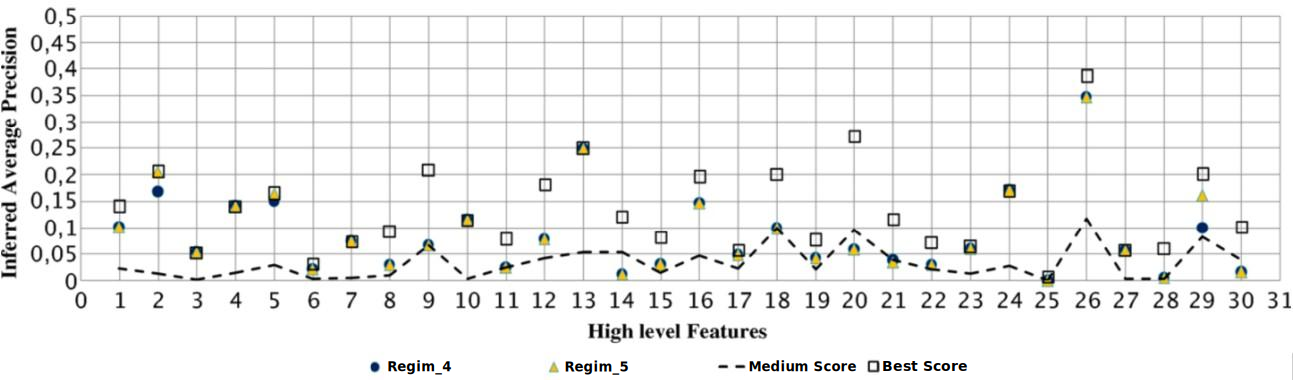
\includegraphics[width=1\textwidth]{graphics/trecvid3}
			\caption{\textit{TrecVid 2010}: $regim_{4}$ and $regim_{5}$ runs evaluations}
			\label{res1tervcid2010}
		\end{figure*}

		With such results, we extended our experimentation on the same dataset by using more rules 
		for the deduction engine. Indeed, the LSCOM ontology is built on a set of semantic concepts
		interrelated by the generalization relationship (\textit{``is a''}). We transformed this 
		relationship into rules. In total, 4383 rules where defined. The table \ref{tablscom} 
		shows some of these generated rules.

			\begin{table*}
				\centering	
				\caption{Sample rules extracted from the LSCOM ontology}
				\label{tablscom}
				\begin{tabular}{lcl} 
					
					\begin{small}\begin{sffamily}LSCOM Generalization Relationships\end{sffamily} 
					\end{small}& &
					\begin{small}\begin{sffamily}Extracted Rule\end{sffamily}\end{small} \\
					\hline
					\begin{small}\textit{Advocate \textbf{is a} Person} \end{small} & $\Longrightarrow$~~ &
						\begin{small}{\sffamily IsRelatedTo}(Advocate,Person)=1\end{small} \\
					\begin{small}\textit{Airport\_Terminal \textbf{is a} Building} \end{small} &  $\Longrightarrow$~~ &
						\begin{small}{\sffamily IsRelatedTo}(Airport\_Terminal,Building)=1\end{small} \\
					\begin{small}\textit{Backpack \textbf{is a} Luggage} \end{small} &  $\Longrightarrow$~~ &
						\begin{small}{\sffamily IsRelatedTo}(Backpack,Luggage)=1\end{small} \\
							
					\hline 
				\end{tabular}
			\end{table*}
		

		Obtained results are displayed in table \ref{lscom2}. Relying on these results, 
		we can conclude that an indexing system effectiveness can be clearly improved through 
		a knowledge-based approach. In fact, extracting and using rules from LSCOM ontology enable
		precision enhancement of about $18$\%. The recall is improved also of about $8$\%.

		\begin{table*}[h]
			\centering
			\caption{Concept detection enhancement applied on \textit{TRECVID 2010} dataset}
			\label{lscom2}
			\begin{tabular}{lp{1.2cm}p{1.2cm}p{1.2cm}p{1.2cm}p{1.2cm}p{1.2cm}}\hline
			\multicolumn{1}{c}{\multirow{2}{*}{\textit{\textbf{Semantic Concepts}}}} & \multicolumn{3}{c}{\textbf{Visual 				Concept Detector}}                                            & \multicolumn{3}{c}{\textbf								{LSCOM}}                                                                         \\ \cline{2-7} 
\multicolumn{1}{c}{}                                                     & \textit{\textbf{InfAP}}   & \textit{\textbf{P}}      & \multicolumn{1}{l|}{\textit{\textbf{R}}} & \textit{\textbf{infAP}}            & \textit{\textbf{P}}               & \textit{\textbf{R~~~~}}               \\ \hline
\multicolumn{1}{l|}{Outdoor}                                             & -                         & 0.52                     & \multicolumn{1}{c|}{0.59}                & -                                  & \textbf{0.88}                     & \textbf{0.77}                     \\
\multicolumn{1}{l|}{Vegetation}                                          & 0.1                       & 0.74                     & \multicolumn{1}{c|}{0.68}                & 0.1                                & 0.74                              & 0.68                              \\
\multicolumn{1}{l|}{Landscape}                                           & -                         & 0.6                      & \multicolumn{1}{c|}{0.79}                & -                                  & 0.6                               & 0.79                              \\
\multicolumn{1}{l|}{Sky}                                                 & -                         & 0.66                     & \multicolumn{1}{c|}{0.9}                 & -                                  & 0.66                              & 0.9                               \\
\multicolumn{1}{l|}{Trees}                                               & -                         & 0.62                     & \multicolumn{1}{c|}{0.72}                & -                                  & 0.62                              & 0.72                              \\
\multicolumn{1}{l|}{Mountain}                                            & -                         & 0.68                     & \multicolumn{1}{c|}{0.8}                 & -                                  & 0.68                              & 0.8                               \\
\multicolumn{1}{l|}{Ground\_Vehicle}                                     & 0.043                     & 0.3                      & \multicolumn{1}{c|}{0.66}                & \textbf{0.18}                      & \textbf{0.6}                      & \textbf{0.73}                     \\
\multicolumn{1}{l|}{Road}                                                & -                         & 0.43                     & \multicolumn{1}{c|}{0.6}                 & -                                  & 0.43                              & 0.6                               \\
\multicolumn{1}{l|}{Car}                                                 & 0.075                     & 0.42                     & \multicolumn{1}{c|}{0.64}                & \textbf{0.17}                      & \textbf{0.58}                     & \textbf{0.73}                     \\
\multicolumn{1}{l|}{Bus}                                                 & -                         & 0.52                     & \multicolumn{1}{c|}{0.73}                & -                                  & 0.52                              & 0.73                              \\
\multicolumn{1}{l|}{Bicycles}                                            & 0.142                     & 0.67                     & \multicolumn{1}{c|}{0.92}                & \textbf{0.185}                     & \textbf{0.82}                     & \textbf{0.97}                     \\
\multicolumn{1}{l|}{Emergency Vehicle}                                   & -                         & 0.9                      & \multicolumn{1}{c|}{0.83}                & -                                  & 0.9                               & 0.83                              \\
\multicolumn{1}{l|}{Building}                                            & 0.022                     & 0.18                     & \multicolumn{1}{c|}{0.22}                & \textbf{0.1}                       & \textbf{0.5}                      & \textbf{0.43}                     \\
\multicolumn{1}{l|}{Truck}                                               & -                         & 0.35                     & \multicolumn{1}{c|}{0.37}                & -                                  & 0.35                              & 0.37                              \\
\multicolumn{1}{l|}{Airplane Flying}                                     & 0.102                     & 0.8                      & \multicolumn{1}{c|}{0.78}                & 0.102                              & 0.8                               & 0.78                              \\
\multicolumn{1}{l|}{Airplane}                                            & -                         & 0.5                      & \multicolumn{1}{c|}{0.6}                 & -                                  & 0.6                               & 0.6                               \\ \hline\hline
\textbf{Total}                                                           & \multicolumn{1}{|l}{0.071}  & 0.53 & \multicolumn{1}{l|}{0.66}                & \multicolumn{1}{l}{\textbf{0.134}} & \multicolumn{1}{l}{\textbf{0.64}} & \multicolumn{1}{l}{\textbf{0.71}} \\ \hline
\end{tabular}
\end{table*}



		In order to investigate further the effectiveness of our approach in semantic concept detection 
		enhancement, we extended our interest to deal with other datasets mainly 
		the \textit{ImageClef 2012} one.


		\begin{table*}[ht!]
			\centering	
			\caption{Distribution of extracted $\mathsf{isRelatedTo}$ roles according to 
			their fuzzy weights and the defined context}
			\label{table:context-based_ontology}
				\begin{tabular}{c l c c c c c c c c c c} \hline
				~&\multirow{3}{*}{\textbf{Detected Contexts}}& \multicolumn{4}{c}{\scriptsize 
						\textbf{Number of extracted fuzzy rules according}}\\
				~& & \multicolumn{4}{c}{\scriptsize  \textbf{to their fuzzy weight intervals}}\\ 		
				~& & \small{$[0, 0.3[$} & \small{$[0.3, 0.5[$} & \small{$[0.5, 0.7[$} & 
				\small{$[0.7, 1.0]$} \\ 		\hline \hline
			\scriptsize{1}&\small{sentiment\_euphoric}	&783	&605	&510	&534\\
			\scriptsize{2}&\small{sentiment\_happy}		&2020	&864	&519	&444\\
			\scriptsize{3}&\small{setting\_sportsrecreation}&1264	&752	&483	&456\\ 
			\scriptsize{4}&\small{age\_child}		&1045	&649	&493	&441\\ 
			\scriptsize{5}&\small{relation\_familyfriends}	&1150	&903	&398	&522\\ \hline
			\scriptsize{86}&\small{fauna\_cat}		&115	&105	&91	&203\\ 
			\scriptsize{87}&\small{fauna\_insect}		&107	&63	&43	&192\\
			\scriptsize{88}&\small{fauna\_rodent}		&43	&53	&43	&139\\ 
			\scriptsize{89}&\small{fauna\_amphibianreptile}	&24	&29	&43	&127\\ 
			\scriptsize{90}&\small{fauna\_spider}		&3	&20	&16	&48\\ \hline \hline
			\multicolumn{2}{c}{\textbf{All contexts}}	&91803 	&50210	&27435	&33667\\
			 \hline \hline
			\multicolumn{2}{c}{\textbf{Total}}& \multicolumn{4}{c}{\textbf{203115 $\mathsf{isRelatedTo}$ 
								roles}}\\ \hline
			\end{tabular}
		\end{table*}


		\section{Experiments with \textit{ImageClef 2012} dataset}


		In this section, we start by showing the evaluation dataset used to measure the semantic interpretation enhancement. 
		Then, we detail contextualized 
		and non-contextualized ontology construction within our framework. Finally, we show our system performance 
		locally (performances of each ontology separately) and globally (performances of all ontologies) against a non 
		ontology based semantic interpretation approach.

		\subsection{Dataset setup}
			In order to test the consistency of our proposed framework, we used a snapshot of the 
			provided dataset in \emph{ImageCLEF2012's Flickr Photo Annotation and Retrieval} \cite{Thomee2012}. 
			This latter is a challenge to test and benchmark novel
			retrieval systems on social shared photos from \emph{Flickr}.
			This image dataset consists of 25 thousand images: 15 thousand for the learning process 
			and 10 thousand for the test one.		
			In addition to the images, 94 semantic concepts are defined referring to many and various 
			subjects (people, nature, events, \dots). 
			The learning image collection of \emph{Flickr} dataset is annotated with 
			binary decisions to depict if a concept is considered to 
			be present ($tf = 1$) or not ($tf = 0$) in an image. 
			
		\subsection{Evaluation metrics}
			In order to be able to compare different indexing approaches, various system effectiveness 
			metrics have been used. These metrics are commonly based on \emph{precision} (which is defined 
			as the number of relevant answers as a part of the total number of retrieved ones), and \emph{recall} 
			(which is defined as the number of relevant answers as part of total relevant ones in the collection). 
			In our work, we consider the two evaluation measures \emph{Mean Average Precision} (\textit{\textbf{map}}) and  
			\emph{Geometric Mean Average Precision} (\textit{\textbf{gmap}}) \cite{Thomee2012} (measurement considered in the 
			\emph{ImageCLEF2012's Flickr Photo Annotation and Retrieval}).

			The \textit{\textbf{map}} ranks
			images by their confidence scores for each concept,
			then interpolates the values to the range from $0.0$ to $1.0$. The two sub-measures \emph{overall 
			non-interpolated MAP} (\textit{\textbf{map$_{n}$}}) 
			and \emph{overall interpolated MAP} (\textit{\textbf{map$_{i}$}})  are computed.

			The \textit{\textbf{gmap}} is 
			considered as an extension to the (\textit{\textbf{map}}) 
			measure as it uses the same computing procedure, but it 's very useful
			when we focus on low performing semantic interpretation for particular concepts.
			The two sub-measures \emph{non-interpolated GMAP} (\textit{\textbf{gmap$_{n}$}}) and
			\emph{interpolated GMAP} (\textit{\textbf{gmap$_{i}$}}) are computed.

		\subsection{Ontologies Populations}
			\subsubsection{Non-contextualized Ontology Population}
		After computing similarities between the 94 concepts to identify $\mathsf{isRelatedTo}$ roles
		within the learning part of the used dataset, the $Abox$ $\mathcal{A}$ of a non-contextualized ontology 
		is populated as pattern $P1$.
		The extraction process delivers the results described in table \ref{table:context-less_ontology}.
		We note that 629 $\mathsf{isRelated}$ roles are defined where the weight is higher than $0.5$.
		The effectiveness of these roles to improve the semantic interpretation 
		will be discussed later in this section.

		%%%%%%%%%%%%%%%%%%%%%%%%%%%%%
		\begin{table}
			\centering	
			\caption{Number of computed  $\mathsf{isRelatedTo}$ roles within the 
				non-contextualized ontology sorted by their fuzzy weights}
			\label{table:context-less_ontology}
			\begin{tabular}{cc} \hline
				\textbf{Weight}& \textbf{Extracted $\mathsf{isRelatedTo}$ roles}\\
				\hline
				\small{$[0.0, 0.3[$}  & 5219\\ 
				\small{$[0.3, 0.5[$}  & 953\\ 
				\small{$[0.5, 0.7[$}  & 344\\
				\small{$[0.7, 1.0[$}  & 285\\ \hline
				\textbf{Total}  & 6801\\ \hline
			\end{tabular}
		\end{table}
		%%%%%%%%%%%%%%%%%%%%%%%%%%%%%

		We enumerate some of $\mathsf{isRelatedTo}$ roles from the described non-contextualized ontology:
		\begin{align*}
 			R1-&(age\_adult,weather\_rainbow):\mathsf{isRelatedTo} \geq 0.02\\
			R2-&(gender\_female,view\_indoor):\mathsf{isRelatedTo} \geq 0.45\\
			R3-&(scape\_mountainhill,view\_outdoor):\mathsf{isRelatedTo} \geq 0.99
		\end{align*}

		
		While the role $R3$ describes a comprehensible relationships
		between the two concepts \emph{mountain hill} and \emph{outdoor view} (with a fuzzy weight of $0.99$), the role $R1$ 
		describes an exceptional case where the existence of an \emph{adult} in a video shot may 
		lead to the existence of a
		\emph{rainbow} in the same shot. Thus, and regarding this exceptional case, the fuzzy weight of 
		this role is $0.05$.


			\subsubsection{Contextualized Ontologies Population}
		In order to populate the context-based ontologies, we start by defining the set of considered contexts. 
		At first, we consider every concept as a context, and then, we look for specific relationships between other 
		concepts within this context. If any relationships are found, the defined concept will be considered
		as a context. 
		By doing so, our proposed platform can provide automatically a set of context to work with. We consider 
		that a context exists in a video shot only if this latter is strongly tagged by that context to a degree equal 
		to or higher than $0.7$. Then, we adjust the value of the threshold $\gamma$ at $0.7$.

		Our experimentation has led to define 90 contexts (from the 94 concepts). 
		Table \ref{table:context-based_ontology} enumerates a partial view of this set of contexts, 
		and shows the first and the last 5 contexts sorted 
		by the number of $\mathsf{isRelatedTo}$ roles with a fuzzy weight equal to or higher than $0.5$.
		Compared to the non-contextualized ontology, the number of roles is slightly greater. But the total number 
		of roles across ontologies is widely higher. This can help us to deduce that the 
		contextualization of relations between concepts can lead to refine and increase 
		the amount of relationships, and therefore, the content of ontologies.
		%%%%%%%%%%%%%%%%%%%%%%%%%%%%%
		\begin{table*}
		\centering	
		\caption{Distribution of extracted $\mathsf{isRelatedTo}$ roles according to their fuzzy weights and the defined context}
		\label{table:context-based_ontology}
		\begin{tabular}{c l c c c c c c c c c c} \hline
		~&\textbf{Context}& \small{$[0, 0.3[$} & \small{$[0.3, 0.5[$} & \small{$[0.5, 0.7[$} & \small{$[0.7, 1.0]$} \\ 
		\hline
			\scriptsize{1}&\small{sentiment\_euphoric}	&783	&605	&510	&534\\
			\scriptsize{2}&\small{sentiment\_happy}		&2020	&864	&519	&444\\
			\scriptsize{3}&\small{setting\_sportsrecreation}&1264	&752	&483	&456\\ 
			\scriptsize{4}&\small{age\_child}		&1045	&649	&493	&441\\ 
			\scriptsize{5}&\small{relation\_familyfriends}	&1150	&903	&398	&522\\ \hline
			\scriptsize{86}&\small{fauna\_cat}		&115	&105	&91	&203\\ 
			\scriptsize{87}&\small{fauna\_insect}		&107	&63	&43	&192\\
			\scriptsize{88}&\small{fauna\_rodent}		&43	&53	&43	&139\\ 
			\scriptsize{89}&\small{fauna\_amphibianreptile}	&24	&29	&43	&127\\ 
			\scriptsize{90}&\small{fauna\_spider}		&3	&20	&16	&48\\ \hline 
			\multicolumn{2}{c}{\textbf{All contexts}}	&91803 	&50210	&27435	&33667\\
			\hline
			\multicolumn{2}{c}{\textbf{Total}}& \multicolumn{10}{c}{\textbf{203115 $\mathsf{isRelatedTo}$ 
								roles for 90 defined contexts}}\\ \hline
		\end{tabular}
		\end{table*}
		%%%%%%%%%%%%%%%%%%%%%%%%%%%%%
		

		Taking some roles as examples, we focus on the contexts \emph{age\_adult}, \emph{transport\_car},
		\emph{setting\_homelife} and \emph{age\_teenager}:
		\begin{equation*}
			\begin{array}{ c c l c l}
			R4 & - &\mathcal{K}^{f}_{age\_adult} 
				& - & (age\_teenager,sentiment\_scary):\mathsf{isRelatedTo} \geq 0.12\\
			R5 & - &\mathcal{K}^{f}_{transport\_car}
				& - & (sentiment\_happy,timeofday\_day):\mathsf{isRelatedTo} \geq 0.95\\
			R6 & - &\mathcal{K}^{f}_{setting\_homelife} 
				& - & (quantity\_biggroup,sentiment\_happy):\mathsf{isRelatedTo} \geq 0.81\\
			R7 & - &\mathcal{K}^{f}_{age\_teenager}
				& - & (sentiment\_funny,quantity\_two):\mathsf{isRelatedTo} \geq 0.48
			
			\end{array}
		\end{equation*}

		The role $R4$ depicts that in the case of a video shot tagged by the concept \emph{age\_teenager} 
		and strongly tagged by the concept \emph{age\_adult} (here considered as a context), then the concept 
		\emph{sentiment\_scary} could exist in the same shot. Naturally, this case is not always true, 
		and this is why the fuzzy weight of this role is very weak ($0.12$).

		Then, the roles $R5$  and $R6$ depict strong relationships between the two concepts 
		\emph{sentiment\_happy} and \emph{timeofday\_day} within the context \emph{transport\_car},
		and between the two concepts \emph{quantity\_ biggroup} and \emph{sentiment\_happy} within 
		the context \emph{setting\_homelife}. These two relationships are considered as strong roles 
		(where the fuzzy weights are higher than $0.8$).

		Finally, and after extracting knowledge from the learning dataset and generating non-contextualized
		and contextualized roles, the pattern $P1$ is fired consisting in, for each ontology :
		\begin{enumerate}
			\item defining the context of the current ontology and inserting
			 it as an individual of the $\mathsf{context}$ class,
			\item inserting the concepts list as individuals for the $\mathsf{Concept}$ class,
			\item instantiating extracted $\mathsf{isRelatedTo}$ roles for the specific context.
		\end{enumerate}
		For the non-contextualized ontology, 
		only steps (2) and (3) are processed. The set of ontologies are so initiated.
		
		We point out that the obtained and discussed number of roles obtained by the knowledge
		extraction process from the video annotation dataset, could not show the effectiveness of our 
		framework. Indeed, we continue to experiment fuzzy reasoning process based 
		on these roles to assess the semantic enrichment in the next section.

		\subsection{Enhancement Evaluation}
		To evaluate our proposed framework, we have compared our results with an image annotation 
		method detailed in \cite{Ksibi2012} within the \emph{Flickr Photo Annotation Task}. 
		This earlier approach detects semantic concepts through extracting
		local low-level feature vectors: \textsc{Sift} and \textsc{Sift-Hsv}.
		Then, it constructs a semantic context network to depict intrinsic 
		contextual information between concepts in order to enhance automatic 
		photo annotation accuracy. In this paper, we explore further the semantic concepts 
		co-existence (from the training annotated dataset) in order to build and populate 
		fuzzy ontologies in an automated manner.
		
		In an effort to assess our fuzzy ontology based approach capabilities, 
		we conducted an annotation accuracy experimentation for the
		two approaches within the \emph{ImageClef'2012 Flickr Photo Annotation and
		Retrieval} task.
		Thus, two runs were evaluated: the first one concerns the evaluation of  
		the image annotation approach. And the second run concerns the evaluation 
		of the enhancement of the first run annotation results through the use of
		our proposed fuzzy ontology based approach.

		%In our work, we are interested in improving this method. Thus, we used the
		% results given by this method as input for our framework looking for enhancing the semantic interpretation and for 
	%	proving the effectiveness of the use of fuzzy contextualized ontology and
		% fuzzy reasoning in video information \revThree{indexing} systems.

		Mathematically, and as input, we have a set of images where each one is tagged by  some 
		semantic concepts from the 94 concepts defined in the \emph{ImageCLEF2012's Flickr Photo 
		Annotation and Retrieval} dataset. Then, as output, we deliver the same set of
		images, but with an improved concept tagging. For the ontology side, this set of images and their 
		related concepts are converted in $Abox$ $\mathcal{A}$ for various contextualized ontologies.
		Then, we proceed image by image through steps depicted by the algorithm \ref{algo11} 
		to prepare the ontologies and launch the fuzzy reasoning engine to enhance the 
		semantic interpretation of each image.

		Let $Input$ and $Output$ be sets of quadruplet $(t_{k},c,shot_{i},(\alpha_{1}, \alpha_{2}))$. 
		Each quadruplet depicts that the shot 
		$shot_{i}$ is tagged by the concept $c$ by a fuzzy weight $\alpha_{2}$ within the context $t_{k}$,
		and tagged by the context $t_{k}$ by a fuzzy weight $\alpha_{1}$.
		These quadruplets are correlated 
		with the $\mathsf{isIndexedBy}$ and $\mathsf{ExistsIn}$ roles ($\langle(t_{k},s): 
		\mathsf{ExistsIn} \geqslant (\alpha_{1})\rangle$ and $\langle(shot_{i},c) : \mathsf{isIndexedBy} 
		\geqslant (\alpha_{2})\rangle$).

		\begin{algorithm}
			\label{algo11}
			\SetAlgoLined
			%\KwData{$Input \neq \emptyset$ and $Output = \emptyset$ }
			%\KwResult{$Output \neq \emptyset$ }
			\For{each context $t_{k}$ ($k \in [1,90]$)}{
				(1) Fire the pattern $P3$ to clean the ontology $\mathcal{K}^{f}_{t_{k}}$\;
				(2) Instantiate from the class $\mathsf{Shot}$ an individual representing the actual 
					image $shot_{i}$\;
				(3) Instantiate the role $\mathsf{ExistsIn}$ between the shot $shot_{i}$ 
					and the context $t_{k}$\;
				(4) Instantiate the role $\mathsf{isIndexedBy}$ between the shot $shot_{i}$ 
					and the concept $c$\;
				(5) Launch the fuzzy reasoning engine on the ontology $\mathcal{K}^{f}_{t_{k}}$ to enhance
					the $Abox$ $\mathcal{A}$ content\;
				(6) Update the $\mathsf{Output}$ set by extended quadruplet based on $\mathsf{isIndexedBy}$
					within the $Abox$ $\mathcal{A}$\;	
			}
			\caption{Algorithm to prepare and launch the fuzzy reasoning within fuzzy 
			ontologies for an image $shot_{i}$}
		\end{algorithm}

		After applying the algorithm \ref{algo11} on all images in the test dataset, the set 
		\emph{output} is ready to be evaluated. So, we used the evaluation tool supplied by \emph{ImageCLEF}
		(\emph{imageclef2012CR}). We have carried out unit evaluations over ontologies 
		(each ontology is evaluated separately). Finally, we applied an overall assessment showing 
		the performance of our framework (all ontologies combined).


		\subsubsection{Unit evaluation}
		In this section, we try to evaluate each ontology separately. In addition, two
		evaluation levels have been carried out. The first one (named \emph{Level1 Test}) is applied to roles with 
		fuzzy weights equal to or higher than $0.5$ , and the second (named \emph{Level2 Test}) is applied to 
		the ones with fuzzy weights equal to or higher than $0.7$. 
		Table \ref{eval::1} displays unit evaluations with four different measurements in 
		\emph{Level1 Test} and \emph{Level2 Test}.
		The first row details the evaluation of the \emph{Input} set (performance of the system detailed in 
		\cite{Ksibi2012}). The next row details the non-contextualized ontology performance evaluation. 
		The rest of the rows describe contextualized ontologies performance evaluation.
		In order to make the table \ref{eval::1} interpretation easier, three styles were used:
		bold values depict enhancing performances compared to the corresponding 
		evaluation in the first row, 
		underlined values depict a decreasing performance, and finally, the non styled values depict same performance 
		as reference. 

		%%%%%%%%%%%%%%%%%%%%%%%%%%%%%
	\begin{center}
	
	\tablefirsthead{%
		\hline
		&	\multicolumn{4}{c}{\small{\emph{Level1 Test} Evaluation}}&
			\multicolumn{4}{c}{\small{\emph{Level2 Test} Evaluation}}\\  \hline
		\small{\textbf{Context}} & \small{\textbf{map$_{n}$}} & \small{\textbf{map$_{i}$}} & 
		\small{\textbf{gmap$_{n}$}}& \small{\textbf{gmap$_{i}$}} &\small{\textbf{map$_{n}$}} & 
		\small{\textbf{map$_{i}$}} & \small{\textbf{gmap$_{n}$}}& \small{\textbf{gmap$_{i}$}}\\
		\hline
	}
	\tablehead{%
		\hline
		&	\multicolumn{4}{c}{\small{\emph{Level1 Test} Evaluation}}&
			\multicolumn{4}{c}{\small{\emph{Level2 Test} Evaluation}}\\  \hline
		\small{\textbf{Context}} & \small{\textbf{map$_{n}$}} & \small{\textbf{map$_{i}$}} & 
		\small{\textbf{gmap$_{n}$}}& \small{\textbf{gmap$_{i}$}} &\small{\textbf{map$_{n}$}} & 
		\small{\textbf{map$_{i}$}} & \small{\textbf{gmap$_{n}$}}& \small{\textbf{gmap$_{i}$}}\\
		\hline
	}
	\tabletail{%
		\hline
		\multicolumn{9}{r}{\small\sl continued on next page}\\
		\hline
	}
	\tablelasttail{\hline}
	%\bottomcaption{Unit performances evaluation}
	\topcaption{Unit performances evaluation}
	\begin{supertabular}{lcccc||cccc}
	\label{eval::1}
	\small{System in \cite{Ksibi2012}} & {\scriptsize{0.1207}} & {\scriptsize{0.126}} & {\scriptsize{0.0737}} & {\scriptsize{0.078}}& {\scriptsize{0.1207}} & {\scriptsize{0.126}} & {\scriptsize{0.0737}} & {\scriptsize{0.078}}\\
\small{Non-contextualized ontology} & \textbf{\scriptsize{0.1221}} & \textbf{\scriptsize{0.1272}} & \underline{\scriptsize{0.0736}} & \textbf{\scriptsize{0.0784}}& \textbf{\scriptsize{0.1239}} & \textbf{\scriptsize{0.1283}} & \textbf{\scriptsize{0.0747}} & \textbf{\scriptsize{0.0789}}\\
\small{age\_adult} & {\scriptsize{0.1207}} & {\scriptsize{0.126}} & {\scriptsize{0.0737}} & {\scriptsize{0.078}}& {\scriptsize{0.1207}} & {\scriptsize{0.126}} & {\scriptsize{0.0737}} & {\scriptsize{0.078}}\\
\small{age\_baby} & \textbf{\scriptsize{0.1213}} & \textbf{\scriptsize{0.1275}} & \textbf{\scriptsize{0.0739}} & \textbf{\scriptsize{0.0787}}& \textbf{\scriptsize{0.1213}} & \textbf{\scriptsize{0.1275}} & \textbf{\scriptsize{0.0739}} & \textbf{\scriptsize{0.0787}}\\
\small{age\_child} & {\scriptsize{0.1207}} & {\scriptsize{0.126}} & {\scriptsize{0.0737}} & {\scriptsize{0.078}}& {\scriptsize{0.1207}} & {\scriptsize{0.126}} & {\scriptsize{0.0737}} & {\scriptsize{0.078}}\\
\small{age\_elderly} & {\scriptsize{0.1207}} & {\scriptsize{0.126}} & {\scriptsize{0.0737}} & {\scriptsize{0.078}}& {\scriptsize{0.1207}} & {\scriptsize{0.126}} & {\scriptsize{0.0737}} & {\scriptsize{0.078}}\\
\small{age\_teenager} & \textbf{\scriptsize{0.121}} & \textbf{\scriptsize{0.1279}} & \textbf{\scriptsize{0.0741}} & \textbf{\scriptsize{0.0793}}& \textbf{\scriptsize{0.121}} & \textbf{\scriptsize{0.1279}} & \textbf{\scriptsize{0.0741}} & \textbf{\scriptsize{0.0793}}\\
\small{celestial\_moon} & \textbf{\scriptsize{0.1211}} & \textbf{\scriptsize{0.1273}} & \textbf{\scriptsize{0.0738}} & \textbf{\scriptsize{0.0787}}& \textbf{\scriptsize{0.1211}} & \textbf{\scriptsize{0.1273}} & \textbf{\scriptsize{0.0738}} & \textbf{\scriptsize{0.0787}}\\
\small{celestial\_stars} & \textbf{\scriptsize{0.1212}} & \textbf{\scriptsize{0.1277}} & \textbf{\scriptsize{0.0738}} & \textbf{\scriptsize{0.0789}}& \textbf{\scriptsize{0.1212}} & \textbf{\scriptsize{0.1277}} & \textbf{\scriptsize{0.0738}} & \textbf{\scriptsize{0.0789}}\\
\small{celestial\_sun} & \textbf{\scriptsize{0.121}} & \textbf{\scriptsize{0.1269}} & \underline{\scriptsize{0.0735}} & \textbf{\scriptsize{0.0786}}& \textbf{\scriptsize{0.121}} & \textbf{\scriptsize{0.1269}} & \underline{\scriptsize{0.0735}} & \textbf{\scriptsize{0.0786}}\\
\small{combustion\_fireworks} & \textbf{\scriptsize{0.1208}} & \textbf{\scriptsize{0.1268}} & {\scriptsize{0.0737}} & \textbf{\scriptsize{0.0785}}& \textbf{\scriptsize{0.1208}} & \textbf{\scriptsize{0.1268}} & {\scriptsize{0.0737}} & \textbf{\scriptsize{0.0785}}\\
\small{combustion\_flames} & \textbf{\scriptsize{0.1209}} & \textbf{\scriptsize{0.1283}} & \underline{\scriptsize{0.0734}} & \textbf{\scriptsize{0.0789}}& \textbf{\scriptsize{0.1209}} & \textbf{\scriptsize{0.1283}} & \underline{\scriptsize{0.0734}} & \textbf{\scriptsize{0.0789}}\\
\small{combustion\_smoke} & \textbf{\scriptsize{0.1216}} & \textbf{\scriptsize{0.1283}} & {\scriptsize{0.0737}} & \textbf{\scriptsize{0.079}}& \textbf{\scriptsize{0.1216}} & \textbf{\scriptsize{0.1283}} & {\scriptsize{0.0737}} & \textbf{\scriptsize{0.079}}\\
\small{fauna\_amphibianreptile} & {\scriptsize{0.1207}} & \textbf{\scriptsize{0.1271}} & {\scriptsize{0.0737}} & \textbf{\scriptsize{0.0785}}& {\scriptsize{0.1207}} & \textbf{\scriptsize{0.1271}} & {\scriptsize{0.0737}} & \textbf{\scriptsize{0.0785}}\\
\small{fauna\_bird} & \underline{\scriptsize{0.1205}} & \textbf{\scriptsize{0.1268}} & \underline{\scriptsize{0.0735}} & \textbf{\scriptsize{0.0784}}& \underline{\scriptsize{0.1205}} & \textbf{\scriptsize{0.1268}} & \underline{\scriptsize{0.0735}} & \textbf{\scriptsize{0.0784}}\\
\small{fauna\_cat} & \textbf{\scriptsize{0.1211}} & \textbf{\scriptsize{0.1282}} & \textbf{\scriptsize{0.0743}} & \textbf{\scriptsize{0.0794}}& \textbf{\scriptsize{0.1211}} & \textbf{\scriptsize{0.1282}} & \textbf{\scriptsize{0.0743}} & \textbf{\scriptsize{0.0794}}\\
\small{fauna\_dog} & \textbf{\scriptsize{0.1209}} & \textbf{\scriptsize{0.1275}} & \textbf{\scriptsize{0.0738}} & \textbf{\scriptsize{0.0788}}& \textbf{\scriptsize{0.1209}} & \textbf{\scriptsize{0.1275}} & \textbf{\scriptsize{0.0738}} & \textbf{\scriptsize{0.0788}}\\
\small{fauna\_fish} & \textbf{\scriptsize{0.1208}} & \textbf{\scriptsize{0.1275}} & \underline{\scriptsize{0.0734}} & \textbf{\scriptsize{0.0788}}& \textbf{\scriptsize{0.1208}} & \textbf{\scriptsize{0.1275}} & \underline{\scriptsize{0.0734}} & \textbf{\scriptsize{0.0788}}\\
\small{fauna\_horse} & \textbf{\scriptsize{0.1209}} & \textbf{\scriptsize{0.1294}} & \underline{\scriptsize{0.0736}} & \textbf{\scriptsize{0.0794}}& \textbf{\scriptsize{0.1209}} & \textbf{\scriptsize{0.1294}} & \underline{\scriptsize{0.0736}} & \textbf{\scriptsize{0.0794}}\\
\small{fauna\_insect} & \textbf{\scriptsize{0.1209}} & \textbf{\scriptsize{0.1274}} & {\scriptsize{0.0737}} & \textbf{\scriptsize{0.0786}}& \textbf{\scriptsize{0.1209}} & \textbf{\scriptsize{0.1274}} & {\scriptsize{0.0737}} & \textbf{\scriptsize{0.0786}}\\
\small{fauna\_rodent} & \textbf{\scriptsize{0.1209}} & \textbf{\scriptsize{0.1268}} & \textbf{\scriptsize{0.0738}} & \textbf{\scriptsize{0.0783}}& \textbf{\scriptsize{0.1209}} & \textbf{\scriptsize{0.1268}} & \textbf{\scriptsize{0.0738}} & \textbf{\scriptsize{0.0783}}\\
\small{fauna\_spider} & \textbf{\scriptsize{0.1209}} & \textbf{\scriptsize{0.1262}} & {\scriptsize{0.0737}} & \textbf{\scriptsize{0.0781}}& \textbf{\scriptsize{0.1209}} & \textbf{\scriptsize{0.1262}} & {\scriptsize{0.0737}} & \textbf{\scriptsize{0.0781}}\\
\small{flora\_flower} & \textbf{\scriptsize{0.1209}} & \textbf{\scriptsize{0.1279}} & \underline{\scriptsize{0.0735}} & \textbf{\scriptsize{0.0792}}& \textbf{\scriptsize{0.1209}} & \textbf{\scriptsize{0.1279}} & \underline{\scriptsize{0.0735}} & \textbf{\scriptsize{0.0792}}\\
\small{flora\_grass} & \textbf{\scriptsize{0.1211}} & \textbf{\scriptsize{0.1275}} & \underline{\scriptsize{0.0735}} & \textbf{\scriptsize{0.0789}}& \textbf{\scriptsize{0.1211}} & \textbf{\scriptsize{0.1275}} & \underline{\scriptsize{0.0735}} & \textbf{\scriptsize{0.0789}}\\
\small{flora\_plant} & \underline{\scriptsize{0.1205}} & \textbf{\scriptsize{0.1283}} & \underline{\scriptsize{0.0733}} & \textbf{\scriptsize{0.0792}}& \underline{\scriptsize{0.1205}} & \textbf{\scriptsize{0.1283}} & \underline{\scriptsize{0.0733}} & \textbf{\scriptsize{0.0792}}\\
\small{flora\_tree} & \underline{\scriptsize{0.063}} & \underline{\scriptsize{0.0622}} & \underline{\scriptsize{0.0272}} & \underline{\scriptsize{0.0254}}& \textbf{\scriptsize{0.121}} & \textbf{\scriptsize{0.1273}} & \underline{\scriptsize{0.0736}} & \textbf{\scriptsize{0.0786}}\\
\small{gender\_female} & \textbf{\scriptsize{0.1216}} & \textbf{\scriptsize{0.1286}} & \textbf{\scriptsize{0.0742}} & \textbf{\scriptsize{0.0796}}& \textbf{\scriptsize{0.1216}} & \textbf{\scriptsize{0.1286}} & \textbf{\scriptsize{0.0742}} & \textbf{\scriptsize{0.0796}}\\
\small{gender\_male} & \textbf{\scriptsize{0.1211}} & \textbf{\scriptsize{0.1275}} & \textbf{\scriptsize{0.074}} & \textbf{\scriptsize{0.0796}}& \textbf{\scriptsize{0.1211}} & \textbf{\scriptsize{0.1275}} & \textbf{\scriptsize{0.074}} & \textbf{\scriptsize{0.0796}}\\
\small{lighting\_lenseffect} & \textbf{\scriptsize{0.1214}} & \textbf{\scriptsize{0.128}} & \textbf{\scriptsize{0.0738}} & \textbf{\scriptsize{0.0789}}& \textbf{\scriptsize{0.1214}} & \textbf{\scriptsize{0.128}} & \textbf{\scriptsize{0.0738}} & \textbf{\scriptsize{0.0789}}\\
\small{lighting\_reflection} & \textbf{\scriptsize{0.1208}} & \textbf{\scriptsize{0.1292}} & \underline{\scriptsize{0.0735}} & \textbf{\scriptsize{0.0794}}& \textbf{\scriptsize{0.1208}} & \textbf{\scriptsize{0.1292}} & \underline{\scriptsize{0.0735}} & \textbf{\scriptsize{0.0794}}\\
\small{lighting\_shadow} & \textbf{\scriptsize{0.1212}} & \textbf{\scriptsize{0.1291}} & {\scriptsize{0.0737}} & \textbf{\scriptsize{0.0792}}& \textbf{\scriptsize{0.1212}} & \textbf{\scriptsize{0.1291}} & {\scriptsize{0.0737}} & \textbf{\scriptsize{0.0792}}\\
\small{lighting\_silhouette} & \underline{\scriptsize{0.1206}} & \textbf{\scriptsize{0.1269}} & \underline{\scriptsize{0.0734}} & \textbf{\scriptsize{0.0786}}& \underline{\scriptsize{0.1206}} & \textbf{\scriptsize{0.1269}} & \underline{\scriptsize{0.0734}} & \textbf{\scriptsize{0.0786}}\\
\small{quality\_artifacts} & \underline{\scriptsize{0.063}} & \underline{\scriptsize{0.0622}} & \underline{\scriptsize{0.0272}} & \underline{\scriptsize{0.0254}}& \textbf{\scriptsize{0.1217}} & \textbf{\scriptsize{0.1286}} & \textbf{\scriptsize{0.074}} & \textbf{\scriptsize{0.0795}}\\
\small{quality\_completeblur} & \textbf{\scriptsize{0.1214}} & \textbf{\scriptsize{0.1286}} & \textbf{\scriptsize{0.0738}} & \textbf{\scriptsize{0.0793}}& \textbf{\scriptsize{0.1214}} & \textbf{\scriptsize{0.1286}} & \textbf{\scriptsize{0.0738}} & \textbf{\scriptsize{0.0793}}\\
\small{quality\_motionblur} & \textbf{\scriptsize{0.1214}} & \textbf{\scriptsize{0.1277}} & \textbf{\scriptsize{0.0741}} & \textbf{\scriptsize{0.0791}}& \textbf{\scriptsize{0.1214}} & \textbf{\scriptsize{0.1277}} & \textbf{\scriptsize{0.0741}} & \textbf{\scriptsize{0.0791}}\\
\small{quality\_partialblur} & \textbf{\scriptsize{0.1211}} & \textbf{\scriptsize{0.1273}} & \textbf{\scriptsize{0.0738}} & \textbf{\scriptsize{0.0786}}& \textbf{\scriptsize{0.1211}} & \textbf{\scriptsize{0.1273}} & \textbf{\scriptsize{0.0738}} & \textbf{\scriptsize{0.0786}}\\
\small{quantity\_biggroup} & \textbf{\scriptsize{0.121}} & \textbf{\scriptsize{0.1273}} & \textbf{\scriptsize{0.0739}} & \textbf{\scriptsize{0.0792}}& \textbf{\scriptsize{0.121}} & \textbf{\scriptsize{0.1273}} & \textbf{\scriptsize{0.0739}} & \textbf{\scriptsize{0.0792}}\\
\small{quantity\_one} & \textbf{\scriptsize{0.1218}} & \textbf{\scriptsize{0.1303}} & \textbf{\scriptsize{0.0745}} & \textbf{\scriptsize{0.0805}}& \textbf{\scriptsize{0.1218}} & \textbf{\scriptsize{0.1303}} & \textbf{\scriptsize{0.0745}} & \textbf{\scriptsize{0.0805}}\\
\small{quantity\_smallgroup} & \textbf{\scriptsize{0.1213}} & \textbf{\scriptsize{0.1276}} & \textbf{\scriptsize{0.0742}} & \textbf{\scriptsize{0.0794}}& \textbf{\scriptsize{0.1213}} & \textbf{\scriptsize{0.1276}} & \textbf{\scriptsize{0.0742}} & \textbf{\scriptsize{0.0794}}\\
\small{quantity\_three} & \textbf{\scriptsize{0.1212}} & \textbf{\scriptsize{0.1271}} & \textbf{\scriptsize{0.0741}} & \textbf{\scriptsize{0.0789}}& \textbf{\scriptsize{0.1212}} & \textbf{\scriptsize{0.1271}} & \textbf{\scriptsize{0.0741}} & \textbf{\scriptsize{0.0789}}\\
\small{quantity\_two} & \textbf{\scriptsize{0.1216}} & \textbf{\scriptsize{0.1284}} & \textbf{\scriptsize{0.0742}} & \textbf{\scriptsize{0.0797}}& \textbf{\scriptsize{0.1216}} & \textbf{\scriptsize{0.1284}} & \textbf{\scriptsize{0.0742}} & \textbf{\scriptsize{0.0797}}\\
\small{relation\_coworkers} & \textbf{\scriptsize{0.1211}} & \textbf{\scriptsize{0.1275}} & \textbf{\scriptsize{0.0741}} & \textbf{\scriptsize{0.0795}}& \textbf{\scriptsize{0.1211}} & \textbf{\scriptsize{0.1275}} & \textbf{\scriptsize{0.0741}} & \textbf{\scriptsize{0.0795}}\\
\small{relation\_familyfriends} & \textbf{\scriptsize{0.1216}} & \textbf{\scriptsize{0.1277}} & \textbf{\scriptsize{0.0745}} & \textbf{\scriptsize{0.0793}}& \textbf{\scriptsize{0.1216}} & \textbf{\scriptsize{0.1277}} & \textbf{\scriptsize{0.0745}} & \textbf{\scriptsize{0.0793}}\\
\small{relation\_strangers} & \textbf{\scriptsize{0.1214}} & \textbf{\scriptsize{0.1282}} & \textbf{\scriptsize{0.074}} & \textbf{\scriptsize{0.0795}}& \textbf{\scriptsize{0.1214}} & \textbf{\scriptsize{0.1282}} & \textbf{\scriptsize{0.074}} & \textbf{\scriptsize{0.0795}}\\
\small{scape\_city} & \textbf{\scriptsize{0.1209}} & \textbf{\scriptsize{0.127}} & \underline{\scriptsize{0.0735}} & \textbf{\scriptsize{0.0785}}& \textbf{\scriptsize{0.1208}} & \underline{\scriptsize{0.1254}} & \underline{\scriptsize{0.0735}} & {\scriptsize{0.078}}\\
\small{scape\_coast} & \textbf{\scriptsize{0.1208}} & \textbf{\scriptsize{0.1269}} & \underline{\scriptsize{0.0732}} & \textbf{\scriptsize{0.0785}}& \textbf{\scriptsize{0.1208}} & \textbf{\scriptsize{0.1269}} & \underline{\scriptsize{0.0732}} & \textbf{\scriptsize{0.0785}}\\
\small{scape\_desert} & \textbf{\scriptsize{0.1211}} & \textbf{\scriptsize{0.1273}} & \underline{\scriptsize{0.0735}} & \textbf{\scriptsize{0.0787}}& \textbf{\scriptsize{0.1211}} & \textbf{\scriptsize{0.1273}} & \underline{\scriptsize{0.0735}} & \textbf{\scriptsize{0.0787}}\\
\small{scape\_forestpark} & \textbf{\scriptsize{0.1212}} & \textbf{\scriptsize{0.1272}} & \textbf{\scriptsize{0.0739}} & \textbf{\scriptsize{0.0788}}& \textbf{\scriptsize{0.1209}} & \textbf{\scriptsize{0.1277}} & {\scriptsize{0.0737}} & \textbf{\scriptsize{0.0792}}\\
\small{scape\_graffiti} & \textbf{\scriptsize{0.1208}} & \textbf{\scriptsize{0.1265}} & \underline{\scriptsize{0.0736}} & \textbf{\scriptsize{0.0784}}& \textbf{\scriptsize{0.1208}} & \textbf{\scriptsize{0.1265}} & \underline{\scriptsize{0.0736}} & \textbf{\scriptsize{0.0784}}\\
\small{scape\_mountainhill} & \textbf{\scriptsize{0.121}} & \textbf{\scriptsize{0.1294}} & \underline{\scriptsize{0.0735}} & \textbf{\scriptsize{0.0801}}& \textbf{\scriptsize{0.121}} & \textbf{\scriptsize{0.1294}} & \underline{\scriptsize{0.0735}} & \textbf{\scriptsize{0.0801}}\\
\small{scape\_rural} & \textbf{\scriptsize{0.1212}} & \textbf{\scriptsize{0.1279}} & \underline{\scriptsize{0.0736}} & \textbf{\scriptsize{0.0792}}& \textbf{\scriptsize{0.1212}} & \textbf{\scriptsize{0.1279}} & \underline{\scriptsize{0.0736}} & \textbf{\scriptsize{0.0792}}\\
\small{sentiment\_active} & \textbf{\scriptsize{0.1218}} & \textbf{\scriptsize{0.1284}} & \textbf{\scriptsize{0.074}} & \textbf{\scriptsize{0.079}}& \textbf{\scriptsize{0.1218}} & \textbf{\scriptsize{0.1284}} & \textbf{\scriptsize{0.074}} & \textbf{\scriptsize{0.079}}\\
\small{sentiment\_calm} & {\scriptsize{0.1207}} & \textbf{\scriptsize{0.1261}} & {\scriptsize{0.0737}} & \textbf{\scriptsize{0.0781}}& {\scriptsize{0.1207}} & \textbf{\scriptsize{0.1261}} & {\scriptsize{0.0737}} & \textbf{\scriptsize{0.0781}}\\
\small{sentiment\_euphoric} & \textbf{\scriptsize{0.1213}} & \textbf{\scriptsize{0.1281}} & \textbf{\scriptsize{0.074}} & \textbf{\scriptsize{0.0794}}& \textbf{\scriptsize{0.1213}} & \textbf{\scriptsize{0.1281}} & \textbf{\scriptsize{0.074}} & \textbf{\scriptsize{0.0794}}\\
\small{sentiment\_funny} & {\scriptsize{0.1207}} & \textbf{\scriptsize{0.1272}} & \underline{\scriptsize{0.0734}} & \textbf{\scriptsize{0.0788}}& {\scriptsize{0.1207}} & \textbf{\scriptsize{0.1272}} & \underline{\scriptsize{0.0734}} & \textbf{\scriptsize{0.0788}}\\
\small{sentiment\_happy} & \textbf{\scriptsize{0.1209}} & \textbf{\scriptsize{0.1274}} & \textbf{\scriptsize{0.0738}} & \textbf{\scriptsize{0.0789}}& \textbf{\scriptsize{0.1209}} & \textbf{\scriptsize{0.1274}} & \textbf{\scriptsize{0.0738}} & \textbf{\scriptsize{0.0789}}\\
\small{sentiment\_inactive} & \textbf{\scriptsize{0.1215}} & \underline{\scriptsize{0.1258}} & \textbf{\scriptsize{0.074}} & \textbf{\scriptsize{0.0784}}& \textbf{\scriptsize{0.1215}} & \textbf{\scriptsize{0.1277}} & \textbf{\scriptsize{0.074}} & \textbf{\scriptsize{0.0788}}\\
\small{sentiment\_melancholic} & \textbf{\scriptsize{0.1215}} & \textbf{\scriptsize{0.1282}} & \textbf{\scriptsize{0.0741}} & \textbf{\scriptsize{0.0791}}& \textbf{\scriptsize{0.1215}} & \textbf{\scriptsize{0.1282}} & \textbf{\scriptsize{0.0741}} & \textbf{\scriptsize{0.0791}}\\
\small{sentiment\_scary} & \textbf{\scriptsize{0.121}} & \textbf{\scriptsize{0.1281}} & \textbf{\scriptsize{0.0738}} & \textbf{\scriptsize{0.0788}}& \textbf{\scriptsize{0.121}} & \textbf{\scriptsize{0.1281}} & \textbf{\scriptsize{0.0738}} & \textbf{\scriptsize{0.0788}}\\
\small{sentiment\_unpleasant} & \textbf{\scriptsize{0.1208}} & \textbf{\scriptsize{0.1269}} & \textbf{\scriptsize{0.0738}} & \textbf{\scriptsize{0.0787}}& \textbf{\scriptsize{0.1208}} & \textbf{\scriptsize{0.1269}} & \textbf{\scriptsize{0.0738}} & \textbf{\scriptsize{0.0787}}\\
\small{setting\_citylife} & \textbf{\scriptsize{0.1215}} & \textbf{\scriptsize{0.1276}} & \textbf{\scriptsize{0.0741}} & \textbf{\scriptsize{0.0789}}& \textbf{\scriptsize{0.1215}} & \textbf{\scriptsize{0.1276}} & \textbf{\scriptsize{0.0741}} & \textbf{\scriptsize{0.0789}}\\
\small{setting\_fooddrink} & \underline{\scriptsize{0.1192}} & \textbf{\scriptsize{0.1273}} & \underline{\scriptsize{0.0728}} & \textbf{\scriptsize{0.079}}& \underline{\scriptsize{0.1206}} & \textbf{\scriptsize{0.1265}} & \underline{\scriptsize{0.0735}} & \textbf{\scriptsize{0.0783}}\\
\small{setting\_homelife} & \textbf{\scriptsize{0.1208}} & \textbf{\scriptsize{0.127}} & {\scriptsize{0.0737}} & \textbf{\scriptsize{0.0786}}& \textbf{\scriptsize{0.1208}} & \textbf{\scriptsize{0.127}} & {\scriptsize{0.0737}} & \textbf{\scriptsize{0.0786}}\\
\small{setting\_partylife} & \textbf{\scriptsize{0.1211}} & \textbf{\scriptsize{0.1272}} & \textbf{\scriptsize{0.0738}} & \textbf{\scriptsize{0.0787}}& \textbf{\scriptsize{0.1211}} & \textbf{\scriptsize{0.1272}} & \textbf{\scriptsize{0.0738}} & \textbf{\scriptsize{0.0787}}\\
\small{setting\_sportsrecreation} & \textbf{\scriptsize{0.1209}} & \textbf{\scriptsize{0.1265}} & \underline{\scriptsize{0.0736}} & \textbf{\scriptsize{0.0783}}& \textbf{\scriptsize{0.1209}} & \textbf{\scriptsize{0.1265}} & \underline{\scriptsize{0.0736}} & \textbf{\scriptsize{0.0783}}\\
\small{style\_circularwarp} & \underline{\scriptsize{0.1204}} & \textbf{\scriptsize{0.127}} & \underline{\scriptsize{0.0733}} & \textbf{\scriptsize{0.0786}}& \underline{\scriptsize{0.1204}} & \textbf{\scriptsize{0.127}} & \underline{\scriptsize{0.0733}} & \textbf{\scriptsize{0.0786}}\\
\small{style\_gray} & \underline{{\scriptsize{0.1206}}} & \textbf{{\scriptsize{0.1271}}} & \underline{{\scriptsize{0.0734}}} & \textbf{{\scriptsize{0.0787}}}& \underline{{\scriptsize{0.1206}}} & \textbf{{\scriptsize{0.1271}}} & \underline{{\scriptsize{0.0734}}} & \textbf{{\scriptsize{0.0787}}}\\
\small{style\_overlay} & \textbf{\scriptsize{0.1211}} & \textbf{\scriptsize{0.1276}} & \textbf{\scriptsize{0.0738}} & \textbf{\scriptsize{0.079}}& \textbf{\scriptsize{0.1211}} & \textbf{\scriptsize{0.1276}} & \textbf{\scriptsize{0.0738}} & \textbf{\scriptsize{0.079}}\\
\small{style\_pictureinpicture} & \textbf{\scriptsize{0.1214}} & \textbf{\scriptsize{0.1272}} & \textbf{\scriptsize{0.0742}} & \textbf{\scriptsize{0.079}}& \textbf{\scriptsize{0.1214}} & \textbf{\scriptsize{0.1272}} & \textbf{\scriptsize{0.0742}} & \textbf{\scriptsize{0.079}}\\
\small{timeofday\_night} & \textbf{\scriptsize{0.1211}} & \textbf{\scriptsize{0.1278}} & \textbf{\scriptsize{0.0738}} & \textbf{\scriptsize{0.0789}}& \textbf{\scriptsize{0.1211}} & \textbf{\scriptsize{0.1278}} & \textbf{\scriptsize{0.0738}} & \textbf{\scriptsize{0.0789}}\\
\small{timeofday\_sunrisesunset} & \textbf{\scriptsize{0.121}} & \textbf{\scriptsize{0.1278}} & \underline{\scriptsize{0.0734}} & \textbf{\scriptsize{0.0789}}& \textbf{\scriptsize{0.121}} & \textbf{\scriptsize{0.1278}} & \underline{\scriptsize{0.0734}} & \textbf{\scriptsize{0.0789}}\\
\small{transport\_air} & \underline{\scriptsize{0.1203}} & \textbf{\scriptsize{0.1262}} & \underline{\scriptsize{0.0734}} & \textbf{\scriptsize{0.0783}}& \underline{\scriptsize{0.1203}} & \textbf{\scriptsize{0.1262}} & \underline{\scriptsize{0.0734}} & \textbf{\scriptsize{0.0783}}\\
\small{transport\_car} & \textbf{\scriptsize{0.1208}} & \textbf{\scriptsize{0.1291}} & \textbf{\scriptsize{0.0738}} & \textbf{\scriptsize{0.0796}}& \textbf{\scriptsize{0.1208}} & \textbf{\scriptsize{0.1291}} & \textbf{\scriptsize{0.0738}} & \textbf{\scriptsize{0.0796}}\\
\small{transport\_cycle} & \textbf{\scriptsize{0.1212}} & \textbf{\scriptsize{0.1277}} & \textbf{\scriptsize{0.0739}} & \textbf{\scriptsize{0.0789}}& \textbf{\scriptsize{0.1212}} & \textbf{\scriptsize{0.1277}} & \textbf{\scriptsize{0.0739}} & \textbf{\scriptsize{0.0789}}\\
\small{transport\_rail} & \textbf{\scriptsize{0.121}} & \textbf{\scriptsize{0.1283}} & \textbf{\scriptsize{0.0739}} & \textbf{\scriptsize{0.0794}}& \textbf{\scriptsize{0.121}} & \textbf{\scriptsize{0.1283}} & \textbf{\scriptsize{0.0739}} & \textbf{\scriptsize{0.0794}}\\
\small{transport\_truckbus} & \textbf{\scriptsize{0.1215}} & \textbf{\scriptsize{0.128}} & \textbf{\scriptsize{0.074}} & \textbf{\scriptsize{0.079}}& \textbf{\scriptsize{0.1215}} & \textbf{\scriptsize{0.128}} & \textbf{\scriptsize{0.074}} & \textbf{\scriptsize{0.079}}\\
\small{transport\_water} & \textbf{\scriptsize{0.1209}} & \textbf{\scriptsize{0.127}} & \underline{\scriptsize{0.0734}} & \textbf{\scriptsize{0.0786}}& \textbf{\scriptsize{0.1209}} & \textbf{\scriptsize{0.127}} & \underline{\scriptsize{0.0734}} & \textbf{\scriptsize{0.0786}}\\
\small{view\_closeupmacro} & {\scriptsize{0.1207}} & \textbf{\scriptsize{0.1268}} & \underline{\scriptsize{0.0735}} & \textbf{\scriptsize{0.0785}}& {\scriptsize{0.1207}} & \textbf{\scriptsize{0.1268}} & \underline{\scriptsize{0.0735}} & \textbf{\scriptsize{0.0785}}\\
\small{view\_indoor} & \textbf{\scriptsize{0.1212}} & \textbf{\scriptsize{0.1283}} & \textbf{\scriptsize{0.0739}} & \textbf{\scriptsize{0.08}}& \textbf{\scriptsize{0.1212}} & \textbf{\scriptsize{0.1283}} & \textbf{\scriptsize{0.0739}} & \textbf{\scriptsize{0.08}}\\
\small{view\_portrait} & \textbf{\scriptsize{0.122}} & \textbf{\scriptsize{0.1279}} & \textbf{\scriptsize{0.0745}} & \textbf{\scriptsize{0.0793}}& \textbf{\scriptsize{0.122}} & \textbf{\scriptsize{0.1279}} & \textbf{\scriptsize{0.0745}} & \textbf{\scriptsize{0.0793}}\\
\small{water\_lake} & \textbf{\scriptsize{0.1213}} & \textbf{\scriptsize{0.1284}} & \textbf{\scriptsize{0.0738}} & \textbf{\scriptsize{0.0791}}& \textbf{\scriptsize{0.1213}} & \textbf{\scriptsize{0.1284}} & \textbf{\scriptsize{0.0738}} & \textbf{\scriptsize{0.0791}}\\
\small{water\_other} & \textbf{\scriptsize{0.121}} & \textbf{\scriptsize{0.1277}} & {\scriptsize{0.0737}} & \textbf{\scriptsize{0.079}}& \textbf{\scriptsize{0.121}} & \textbf{\scriptsize{0.1277}} & {\scriptsize{0.0737}} & \textbf{\scriptsize{0.079}}\\
\small{water\_riverstream} & \textbf{\scriptsize{0.1213}} & \textbf{\scriptsize{0.1275}} & \textbf{\scriptsize{0.0738}} & \textbf{\scriptsize{0.0789}}& \textbf{\scriptsize{0.1213}} & \textbf{\scriptsize{0.1275}} & \textbf{\scriptsize{0.0738}} & \textbf{\scriptsize{0.0789}}\\
\small{water\_seaocean} & \textbf{\scriptsize{0.1214}} & \textbf{\scriptsize{0.1277}} & \textbf{\scriptsize{0.0738}} & \textbf{\scriptsize{0.0788}}& \textbf{\scriptsize{0.1214}} & \textbf{\scriptsize{0.1277}} & \textbf{\scriptsize{0.0738}} & \textbf{\scriptsize{0.0788}}\\
\small{water\_underwater} & \textbf{\scriptsize{0.1208}} & \textbf{\scriptsize{0.1266}} & \underline{\scriptsize{0.0735}} & \textbf{\scriptsize{0.0784}}& \textbf{\scriptsize{0.1208}} & \textbf{\scriptsize{0.1266}} & \underline{\scriptsize{0.0735}} & \textbf{\scriptsize{0.0784}}\\
\small{weather\_clearsky} & \underline{\scriptsize{0.1202}} & \textbf{\scriptsize{0.1281}} & \underline{\scriptsize{0.0735}} & \textbf{\scriptsize{0.0794}}& \textbf{\scriptsize{0.121}} & \textbf{\scriptsize{0.127}} & \textbf{\scriptsize{0.0738}} & \textbf{\scriptsize{0.0785}}\\
\small{weather\_cloudysky} & \textbf{\scriptsize{0.1212}} & \textbf{\scriptsize{0.1272}} & \textbf{\scriptsize{0.0738}} & \textbf{\scriptsize{0.0787}}& \textbf{\scriptsize{0.1212}} & \textbf{\scriptsize{0.1272}} & \textbf{\scriptsize{0.0738}} & \textbf{\scriptsize{0.0787}}\\
\small{weather\_fogmist} & \textbf{\scriptsize{0.1211}} & \textbf{\scriptsize{0.1281}} & {\scriptsize{0.0737}} & \textbf{\scriptsize{0.079}}& \underline{\scriptsize{0.1197}} & \underline{\scriptsize{0.1256}} & \underline{\scriptsize{0.0729}} & \underline{\scriptsize{0.0776}}\\
\small{weather\_lightning} & \textbf{\scriptsize{0.1209}} & \textbf{\scriptsize{0.1277}} & {\scriptsize{0.0737}} & \textbf{\scriptsize{0.0794}}& \textbf{\scriptsize{0.1209}} & \textbf{\scriptsize{0.1277}} & {\scriptsize{0.0737}} & \textbf{\scriptsize{0.0794}}\\
\small{weather\_overcastsky} & {\scriptsize{0.1207}} & \textbf{\scriptsize{0.127}} & \underline{\scriptsize{0.0736}} & \textbf{\scriptsize{0.0785}}& {\scriptsize{0.1207}} & \textbf{\scriptsize{0.127}} & \underline{\scriptsize{0.0736}} & \textbf{\scriptsize{0.0785}}\\
\small{weather\_rainbow} & \textbf{\scriptsize{0.1208}} & \textbf{\scriptsize{0.1274}} & \underline{\scriptsize{0.0735}} & \textbf{\scriptsize{0.0787}}& \textbf{\scriptsize{0.1208}} & \textbf{\scriptsize{0.1274}} & \underline{\scriptsize{0.0735}} & \textbf{\scriptsize{0.0787}}\\
\small{weather\_snowice} & \textbf{\scriptsize{0.1211}} & \textbf{\scriptsize{0.1281}} & \underline{\scriptsize{0.0736}} & \textbf{\scriptsize{0.0795}}& \textbf{\scriptsize{0.121}} & \textbf{\scriptsize{0.1263}} & \underline{\scriptsize{0.0736}} & \textbf{\scriptsize{0.0791}}\\



\end{supertabular}
\end{center}
		%%%%%%%%%%%%%%%%%%%%%%%%%%%%%
		
		%%%%%%%%%%%%%%%%%%%%%%%%%%%%%
		%\input{tables/table4}
		%%%%%%%%%%%%%%%%%%%%%%%%%%%%%

		In table \ref{table_resume1} and \ref{table_resume2}, we computed the semantic 
		enhancement performance for the best and worst 5 cases for both \emph{Level1 Test} and \emph{Level2 Test}
		from the evaluation in table \ref{eval::1}. We observe that some fuzzy 
		ontologies show a semantic enhancement up to $3.4\%$. In particular, the non-contextualized
		ontology shows an increasing performance of $2,65\%$ in \emph{Level2 Test}. This can be due to 
		the large number of roles within the non-contextualized ontology compared with a contextualized one 
		(see table \ref{table:context-less_ontology} and table \ref{table:context-based_ontology}).
		These enhancements are minimal, but still precious. However, some other ontologies have shown a decrease in
		performance. This could be due to non validated and erroneous roles.
		
		Generally, tables \ref{table_resume1} and \ref{table_resume2} prove that our framework could enhance 
		a semantic interpretation. Fuzzy ontologies where the performances decreased will be analyzed later 
		to validate their content by experts. Moreover, \emph{Level1 Test} has shown a very close performances 
		compared to \emph{Level2 Test}. The latter stands out for less performance degradation.
		
		
		%%%%%%%%%%%%%%%%%%%%%%%%%%%%%
		\begin{table*}
	\centering	
	\caption{\textbf{\textit{map$_{n}$}} evaluation performances}
		\label{table_resume1}
		\begin{tabular}{rl rl c} 
			\hline
			
			\multicolumn{2}{c}{\textbf{\textit{map$_{n}$}} (\emph{Level1 Test})} & 
			\multicolumn{2}{c}{\textbf{\textit{map$_{n}$}} (\emph{Level2 Test})} & \\
			\hline  
			Non-contextualized & \textbf{1,16\%}&Non-contextualized &\textbf{2,65\%}& 
			\multirow{5}{*}{5 best evaluations}\\
			view\_portrait&\textbf{1,08\%}&view\_portrait&\textbf{1,08\%}& \\
			quantity\_one&\textbf{0,91\%}&quantity\_one&\textbf{0,91\%}& \\
			sentiment\_active&\textbf{0,91\%}&sentiment\_active&\textbf{0,91\%}& \\
			quantity\_two&\textbf{0,75\%}&quality\_artifacts&\textbf{0,83\%}& \\
			\hline
			transport\_air&\textbf{-0,33\%}&flora\_plant&\textbf{-0,17\%}& \multirow{5}{*}{5 least evaluations}\\
			weather\_clearsky&\textbf{-0,41\%}&fauna\_bird&\textbf{-0,17\%}& \\
			setting\_fooddrink&\textbf{-1,24}\%&style\_circularwarp&\textbf{-0,25\%}& \\
			quality\_artifacts&\textbf{-47,80\%}&transport\_air&\textbf{-0,33\%}& \\
			flora\_tree&\textbf{-47,80\%}&weather\_fogmist&\textbf{-0,83\%}& \\
			\hline 
\end{tabular}
\end{table*}
		%%%%%%%%%%%%%%%%%%%%%%%%%%%%%

		%%%%%%%%%%%%%%%%%%%%%%%%%%%%%
		\begin{table*}
	\centering	
	\caption{\textbf{\textit{map$_{i}$}} evaluation performances}
		\label{table_resume2}
		\begin{tabular}{rl rl c} 
			\hline
			
			\multicolumn{2}{c}{\textbf{\textit{map$_{i}$}} (\emph{Level1 Test})} & 
			\multicolumn{2}{c}{\textbf{\textit{map$_{i}$}} (\emph{Level2 Test})} & \\
			\hline  

			quantity\_one&\textbf{3,41\%}&quantity\_one&\textbf{3,41\%}& \multirow{5}{*}{5 best evaluations}\\
			scape\_mountainhill&\textbf{2,70\%}&scape\_mountainhill&\textbf{2,70\%}& \\
			fauna\_horse&\textbf{2,70\%}&fauna\_horse&\textbf{2,70\%}& \\
			lighting\_reflection&\textbf{2,54\%}&lighting\_reflection&\textbf{2,54\%}& \\
			lighting\_shadow&\textbf{2,46\%}&lighting\_shadow&\textbf{2,46\%}& \\
			\hline
			age\_child&\textbf{0,00\%}&age\_adult&\textbf{0,00\%}& \multirow{5}{*}{5 least evaluations}\\
			age\_elderly&\textbf{0,00\%}&age\_child&\textbf{0,00\%}& \\
			sentiment\_inactive&\textbf{-0,16\%}&age\_elderly&\textbf{0,00\%}& \\
			quality\_artifacts&\textbf{-50,63\%}&weather\_fogmist&\textbf{-0,32\%}& \\
			flora\_tree&\textbf{-50,63\%}&scape\_city&\textbf{-0,48\%}& \\
			\hline 
\end{tabular}
\end{table*}
		%%%%%%%%%%%%%%%%%%%%%%%%%%%%%

		%%%%%%%%%%%%%%%%%%%%%%%%%%%%%
		\begin{table*}
	\centering	
	\caption{\textbf{\textit{gmap$_{n}$}} evaluation performances}
		\label{table_resume3}
		\begin{tabular}{rl rl c} 
			\hline
			
			\multicolumn{2}{c}{\textbf{\textit{gmap$_{n}$}} (\emph{Level1 Test})} & 
			\multicolumn{2}{c}{\textbf{\textit{gmap$_{n}$}} (\emph{Level2 Test})} & \\
			\hline  
			%%%%%%%%%%%%%%%%%%%%%%%%%%%%%%%%%%%%%%%%%%%%%%%%%%%%%%%%%%%%%%%%%%%%%%%%%%%%%%%%%%%%%%
			%%%%%%%%%%%%%%%%%%%%%%%%%%%%%%%%%%%%%%%%%%%%%%%%%%%%%%%%%%%%%%%%%%%%%%%%%%%%%%%%%%%%%%
			%%%%%%%%%%%%%%%%%%%%%%%%%%%%%%%%%%%%%%%%%%%%%%%%%%%%%%%%%%%%%%%%%%%%%%%%%%%%%%%%%%%%%%			
	%quantity\_one&\textbf{1,09\%}&Non-contextualized &\textbf{1,36\%}& \multirow{5}{*}{5 best evaluations}\\
	quantity\_one&\textbf{1,09\%}&Non-contextualized &\textbf{1,36\%}&
	\multirow{5}{*}{5 best evaluations}\\
			%%%%%%%%%%%%%%%%%%%%%%%%%%%%%%%%%%%%%%%%%%%%%%%%%%%%%%%%%%%%%%%%%%%%%%%%%%%%%%%%%%%%%%
			%%%%%%%%%%%%%%%%%%%%%%%%%%%%%%%%%%%%%%%%%%%%%%%%%%%%%%%%%%%%%%%%%%%%%%%%%%%%%%%%%%%%%%
			%%%%%%%%%%%%%%%%%%%%%%%%%%%%%%%%%%%%%%%%%%%%%%%%%%%%%%%%%%%%%%%%%%%%%%%%%%%%%%%%%%%%%%
			
			view\_portrait&\textbf{1,09\%}&quantity\_one&\textbf{1,09\%}& \\
			relation\_familyfriends&\textbf{1,09\%}&view\_portrait&\textbf{1,09\%}& \\
			fauna\_cat&\textbf{0,81\%}&relation\_familyfriends&\textbf{1,09\%}& \\
			gender\_female&\textbf{0,68\%}&fauna\_cat&\textbf{0,81\%}& \\
			\hline
			transport\_air&\textbf{-0,54\%}&flora\_plant&\textbf{-0,41\%}& \multirow{5}{*}{5 least evaluations} \\
			flora\_plant&\textbf{-0,68\%}&fauna\_bird&\textbf{-0,54\%}& \\
			style\_circularwarp&\textbf{-1,22\%}&style\_circularwarp&\textbf{-0,54\%}& \\
			scape\_coast&\textbf{-63,09\%}&transport\_air&\textbf{-0,68\%}& \\
			weather\_fogmist&\textbf{-63,09\%}&weather\_fogmist&\textbf{-1,09\%}& \\
			\hline 
\end{tabular}
\end{table*}
		%%%%%%%%%%%%%%%%%%%%%%%%%%%%%

		%%%%%%%%%%%%%%%%%%%%%%%%%%%%%
		\begin{table*}
	\centering	
	\caption{\textbf{\textit{gmap$_{i}$}} evaluation performances}
		\label{table_resume4}
		\begin{tabular}{rl rl c} 
			\hline
			
			\multicolumn{2}{c}{\textbf{\textit{gmap$_{i}$}} (\emph{Level1 Test})} & 
			\multicolumn{2}{c}{\textbf{\textit{gmap$_{i}$}} (\emph{Level2 Test})} & \\
			\hline  
	
			quantity\_one&\textbf{3,21\%}&quantity\_one&\textbf{3,21\%}& \multirow{5}{*}{5 best evaluations}\\
			scape\_mountainhill&\textbf{2,69\%}&scape\_mountainhill&\textbf{2,69\%}& \\
			view\_indoor&\textbf{2,56\%}&view\_indoor&\textbf{2,56\%}& \\
			quantity\_two&\textbf{2,18\%}&quantity\_two&\textbf{2,18\%}& \\
			gender\_female&\textbf{2,05\%}&gender\_female&\textbf{2,05\%}& \\
			\hline
			age\_adult&\textbf{0,00\%}&scape\_city&\textbf{0,00\%}& \multirow{5}{*}{5 least evaluations} \\
			age\_child&\textbf{0,00\%}&age\_adult&\textbf{0,00\%}& \\
			age\_elderly&\textbf{0,00\%}&age\_child&\textbf{0,00\%}& \\
			quality\_artifacts&\textbf{-67,44\%}&age\_elderly&\textbf{0,00\%}& \\
			flora\_tree&\textbf{-67,44\%}&weather\_fogmist&\textbf{-0,51\%}& \\
			\hline 
\end{tabular}
\end{table*}
		%%%%%%%%%%%%%%%%%%%%%%%%%%%%%

		The above computed performances use the mean average measurement \textbf{\textit{ma}p}. 
		But the \textbf{\textit{gmap}} is 
		very useful in case we focus on low performing semantic interpretation 
		where scores are close to $0.0$. Table \ref{table_resume3} and \ref{table_resume4} show that a considerable 
		improvement has been made by our framework for concept detection by some contextualized ontologies. 
		Indeed, ontologies referred to contexts \emph{quantity\_one}, \emph{view\_Portrait}, 
		\emph{Relationship\_familyfriends}, \emph{gender\_female} and \emph{quantity\_two} have higher 
		\textbf{\textit{gmap}} scores, so some concepts have been significantly  
		emphasized compared to the initial semantic interpretation (within the $Input$ set).

		Finally, the unit evaluation demonstrates the effectiveness of most of the 
		fuzzy ontologies in improving a given semantic interpretation. Ontology evolving 
		will be addressed to handle particular cases where performances decreased. While the above 
		assessments are done on every ontology separately, we discuss the performance 
		of the overall  proposed framework in the next section (all ontologies combined).

		\subsubsection{Overall evaluation}
		The overall assessment consists in evaluating the proposed framework using all 
		constructed ontologies combined. The performance will be related to all the system and not 
		for a particular ontology.
		As in the unit assessment, we consider the two $Input$ and $Output$ sets: while the first set contains 
		the initial semantic interpretation, the second one contains the enhanced semantic 
		interpretation. To compute the $Output$ set, we proceed as detailed in algorithm \ref{algo11} where all 
		ontologies are used in a pipeline. 

		%%%%%%%%%%%%%%%%%%%%%%%%%%%%%
		\begin{table*}
	\centering	
	\caption{Overall performance evaluation}
		\label{final}
		\begin{tabular}{p{4cm}|cc|cc|cc|cc} 
			
			&\multicolumn{2}{c}{\textbf{\textit{map$_{n}$}}} & 
			\multicolumn{2}{c}{\textbf{\textit{map$_{i}$}}} &
			\multicolumn{2}{c}{\textbf{\textit{gmap$_{n}$}}} & 
			\multicolumn{2}{c}{\textbf{\textit{gmap$_{i}$}}}  \\
			& value & \% & value & \% & value  & \% & value & \% \\
			\hline  
		
			Our framework (\emph{Level1 Test} ) & 
						$0,1232$ & \textbf{2.07} & 
						$0,1325$ & \textbf{5.16} & 
						$0,0733$ & \textbf{-0.54} & 
						$0,0808$ & \textbf{3.59} \\
			Our framework (\emph{Level2 Test}) & 
						$0,1232$ & \textbf{2.07} & 
						$0,1324$ & \textbf{5.08} & 
						$0,0732$ & \textbf{-0.68} &
						$0,0807$ & \textbf{3.46} \\
			System in \cite{Ksibi2012}  & $0.1207$ & - & $0.126$ & - & $0.0737$ 
						& - & $0.078$ & - \\

			\hline 
\end{tabular}
\end{table*}
		%%%%%%%%%%%%%%%%%%%%%%%%%%%%%
		
		Table \ref{final} illustrates the semantic interpretation enhancement performance for our 
		proposed ontology based framework.
		Analyzing \textbf{\textit{map$_{n}$}} and \textbf{\textit{map$_{i}$}}
		values in table \ref{final}, our proposed framework delivers a semantic 
		interpretation enhancement at (respectively) $2.07\%$ and $5.16\%$ within \emph{Level1 Test},
		and $2.07\%$ and $5.08\%$ within \emph{Level2 Test}.  While these results prove the effectiveness 
		of our system, it shows that unlike the unit assessment, \emph{Level1 Test} delivers more accurate 
		results than in \emph{Level2 Test}. Furthermore, decreasing \textbf{\textit{gmap$_{n}$}} performance 
		(for both \emph{Level1 Test} and \emph{Level2 Test})
		illustrates the inability of our framework to enhance particular concepts like \emph{flora\_tree} and 
		\emph{quality\_artifacts}.

		While the overall performance of our proposed framework  seems to be interesting, some points
		discussed in the two sections above have to be addressed. Indeed, the decreasing performance for 
		a particular concept detection should be rectified. We point out that the contents of the set 
		of the ontologies are built through an automatic knowledge discovery on an annotated learning 
		dataset. Thus, the knowledge discovery quality is related to the leaning dataset quality, 
		and the quality of the annotation process. This means that eventual erroneous annotations 
		can affect our ontologies content quality, then the overall system performance. 
		Dealing with these situations, we propose to evolve 
		the ontologies content through expert validation 
		in order to increase the performance and then enhance more the semantic interpretation.
		

\subsection{System scalability}
		After effectiveness discussion, we now experiment our approach scalability.
		To develop our framework, we used the database management system
		\textsc{PostgreSql} (v. 9.1) and its procedural language
		\textsc{PL-pgSql}.
		Table {\ref{table_scalabilite}} illustrates the load required to
		perform extracting knowledge from the \emph{ImageClef 2012} photo
		annotated dataset, and to apply a fuzzy reasoning (within both \emph{Level1}
		and \emph{Level2} $\mathsf{isRelatedTo}$ role selection) on a semantic interpretation of a video
		shot. We applied our experiments on a modern desktop machine with a dual-core
		processor and 4 GB of RAM. 
		
		For the fuzzy reasoning process, a processor core is used at
		$100\%{}$ during inferring new Knowledge step. 
		And for extracting knowledge from an annotated video dataset, 
		both the two processor cores use is balancing between $40\%{}$ and $80\%{}$.
		In terms of RAM memory use, we have not seen a large memory 
		allocation for both tasks. 
		This is caused by a adjustable amount of cache memory  
		handled by the \textsc{PostgreSql} system. We conclude that optimized 
		\textsc{PL-pgSql} code allowed gaining a comprehensive knowledge extraction
		load with respect to the amount of extracted knowledge.
		
		Moreover, we note that the performance of the fuzzy 
		reasoning algorithm gave the same execution rate with the use of 
		\emph{Level1}, containing 61731 $\mathsf{isRelatedTo}$ roles, and 
		\emph{Level2}, containing 33952 $\mathsf{isRelatedTo}$ roles (see table
		{\ref{table:context-based_ontology}}). This can be interpreted as follows:
		with doubling $\mathsf{isRelatedTo}$ roles, the system kept the same computing
		rate and load to reasoning with knowledge. 
		Thus, we can conclude that our approach can be considered as scalable.
		
		\begin{table}
			\centering	
			\caption{Our Approach Computing Load}
			\label{table_scalabilite}
			\begin{tabular}{p{4.5cm}|c|p{4cm}}
			\textbf{\textsf{Task}} & \textbf{\textsf{Computing Time}} &
			\textbf{\textsf{Rate}}
			\\
			\hline
   			Knowlege extraction ($\mathsf{isRelatedTo}$ roles)  &
   						01h:19min:14s & 
   						52,82 seconds/ontology (of one context)\\\hline\hline
   			Fuzzy reasoning : \emph{Level2} $\mathsf{isRelatedTo}$ roles selection
   			   			&  	03h:38min:44s      &
   			   			firing 2,36 $\mathsf{isRelatedTo}$ roles/second \\\hline
   			Fuzzy reasoning : \emph{Level1} $\mathsf{isRelatedTo}$ roles selection &
   						07h:31min:52s      &
   						firing 2,28 $\mathsf{isRelatedTo}$
   						roles/second \\\hline
    		\end{tabular}
		\end{table}
		
		

		\subsection{The Ontology Evolving Evaluation}
		Performance computed in the unit and overall evaluations was based on knowledge extraction 
		from a video/image annotated database. 
		Despite the promising results, the fuzzy ontologies content can 
		be improved through experts validation. 
		In this section, we discuss how could this validation process improve 
		the accuracy of obtained semantic enhancement. 
		Thus, we applied an evolving process for two contextualized ontologies of the contexts 
		\emph{View\_portrait} and \emph{quantity\_one}. 
		Two experts inspected and validated about 800 $\mathsf{isRelatedTo}$ roles related to these ontologies. 

		Table \ref{ff} displays obtained results from the evolved ontologies against the original 
		ones (evaluations from table \ref{eval::1}). With a small performance decrease of 
		the context \emph{View\_portrait} ($-0.08\%$), the evolving process has slightly increase 
		the performances of the two contextualized ontologies in term of \textit{\textbf{gmap}}.
		Indeed, the \emph{Level1 Test} gains accurate results for the context \emph{quantity\_one} 
		against the \emph{Level2 Test}. Weak $\mathsf{isRelatedTo}$ roles (with a fuzzy weight between $0.7$ and $0.3$)
		related to this context were more validated than strong ones ( fuzzy weight between $1.0$ and $0.7$). 
		However, strong $\mathsf{isRelatedTo}$ roles related to the context \emph{View\_portrait} 
		were more validated than weak ones.

		With a preliminary experimentation of the evolving process, we could conclude that 
		the ontology evolving could enhance the fuzzy ontologies content, and consequently the semantic interpretation.
		
		%%%%%%%%%%%%%%%%%%%%%%%%%%%%%
		\begin{table*}
	\centering	
	\caption{Evolving performance evaluation}
		\label{ff}
		\begin{tabular}{p{4cm}|cc|cc|cc|cc} 
			
			&\multicolumn{2}{c}{\textbf{\textit{map$_{n}$}}} & 
			\multicolumn{2}{c}{\textbf{\textit{map$_{i}$}}} &
			\multicolumn{2}{c}{\textbf{\textit{gmap$_{n}$}}} & 
			\multicolumn{2}{c}{\textbf{\textit{gmap$_{i}$}}}  \\
			Evolved Ontologies& value & \% & value & \% & value  & \% & value & \% \\
			\hline  
		View\_portrait (\emph{Level1 Test})
		& $0,1219$ & \textbf{-0.08} & $0,1279$ & \textbf{0.00} & $0,0745$ & \textbf{0.00} & $0,0793$ & \textbf{0.00} \\
		quantity\_one (\emph{Level1 Test})
		& $0,1218$ & \textbf{0.00} & $0,1305$ & \textbf{0.15} & $0,0749$ & \textbf{0.54} & $0,0809$ & \textbf{0.50} \\
		\hline
		View\_portrait (\emph{Level2 Test})
		& $0,122$ & \textbf{0.00} & $0,1278$ & \textbf{-0.08} & $0,0746$ & \textbf{0.27} & $0,0793$ & \textbf{0.25} \\
		quantity\_one (\emph{Level2 Test})
		& $0,1218$ & \textbf{0.00} & $0,1304$ & \textbf{0.08} & $0,0748$ & \textbf{0.40} & $0,0808$ & \textbf{0.37} \\
		\hline 
\end{tabular}
\end{table*}
		

\section{Conclusion}

Despite the promising obtained results by our preliminary evaluations, it still some
potential works to be achieved for future improvement. At first, defining ontologies
content was based on computing similarities between concepts granted by a large
annotated images dataset. More advanced fuzzy similarity functions could be addressed in order to handle real fuzzy knowledge to be inserted in proposed ontologies. Then, ontology evolution task could enhance significantly ontology semantic capabilities, and then a semantic interpretation. Thus, we believe that
ontology evolution is a challenging task that we could follow in our future work.
	
